\chapter{Results and discussion from laboratory testing}\label{chap:Results&Disc}


\begin{table}
\centering
\caption{Soil parameters}
\begin{tabular}{c|cc}
\toprule
\multicolumn{1}{l}{}                    & \multicolumn{1}{c}{\textbf{Parameter}} & \textbf{Mean ± Std. Dev} \\ \midrule
\multicolumn{1}{l}{\textbf{}}           & pH (H\textsubscript{2}O)               & 5.384 ± 0.016              \\
\multicolumn{1}{l}{}                    & pH (0.01 M CaCl\textsubscript{2})      & 4.364 ± 0.01               \\
\multicolumn{1}{l}{\textbf{}}           & C-org (\%)                             & 1.315 ± 0.029              \\
\multicolumn{1}{l}{\textbf{}}           & N-tot (\%)                             & 0.106 ± 0.003              \\ \midrule
\multirow{7}{*}{\rotatebox[origin=c]{90}{Exchangeable ions}}      & Al3+         & 0.871 ± 0.011              \\
                                        & H\textsuperscript{+}                   & 0.088 ± 0.029              \\
                                        & Mg\textsuperscript{2+}                 & 0.07 ± 0.001               \\
                                        & Ca\textsuperscript{2+}                 & 1.543 ± 0.026              \\
                                        & Na\textsuperscript{+}                  & 0.009 ± 0                  \\
                                        & K\textsuperscript{+}                   & 0.046 ± 0                  \\
                                        & CEC                                    & 2.627 ± 0.065              \\ \midrule
\multirow{15}{*}{\rotatebox[origin=c]{90}{Total concentration}} & Ba             & 11.033 ± 0.306             \\
                                        & Be                                     & 0.269 ± 0.004              \\
                                        & Cd                                     & 0.195 ± 0.063              \\
                                        & Co                                     & 2.073 ± 0.09               \\
                                        & Cr                                     & 6.127 ± 0.429              \\
                                        & Cu                                     & 9.103 ± 1.142              \\
                                        & Fe                                     & 6740 ± 445.421             \\
                                        & Hg                                     & \textless{}1             \\
                                        & Mn                                     & 123.667 ± 6.807            \\
                                        & Ni                                     & 3.093 ± 0.199              \\
                                        & P                                      & 525.333 ± 29.28           \\
                                        & Pb                                     & 8.450 ± 0.526               \\
                                        & Sr                                     & 6.8 ± 0.668                \\
                                        & V                                      & 12.667 ± 0.874             \\
                                        & Zn                                     & 22.2 ± 1.3                \\ \bottomrule
\end{tabular}
\end{table}
\section{Methods}
Precipitation of a brown fluff was observed when filtered batch tests containing soil was adjusted to pH 3 with 1 M acetic acid

\begin{figure}
    \centering
    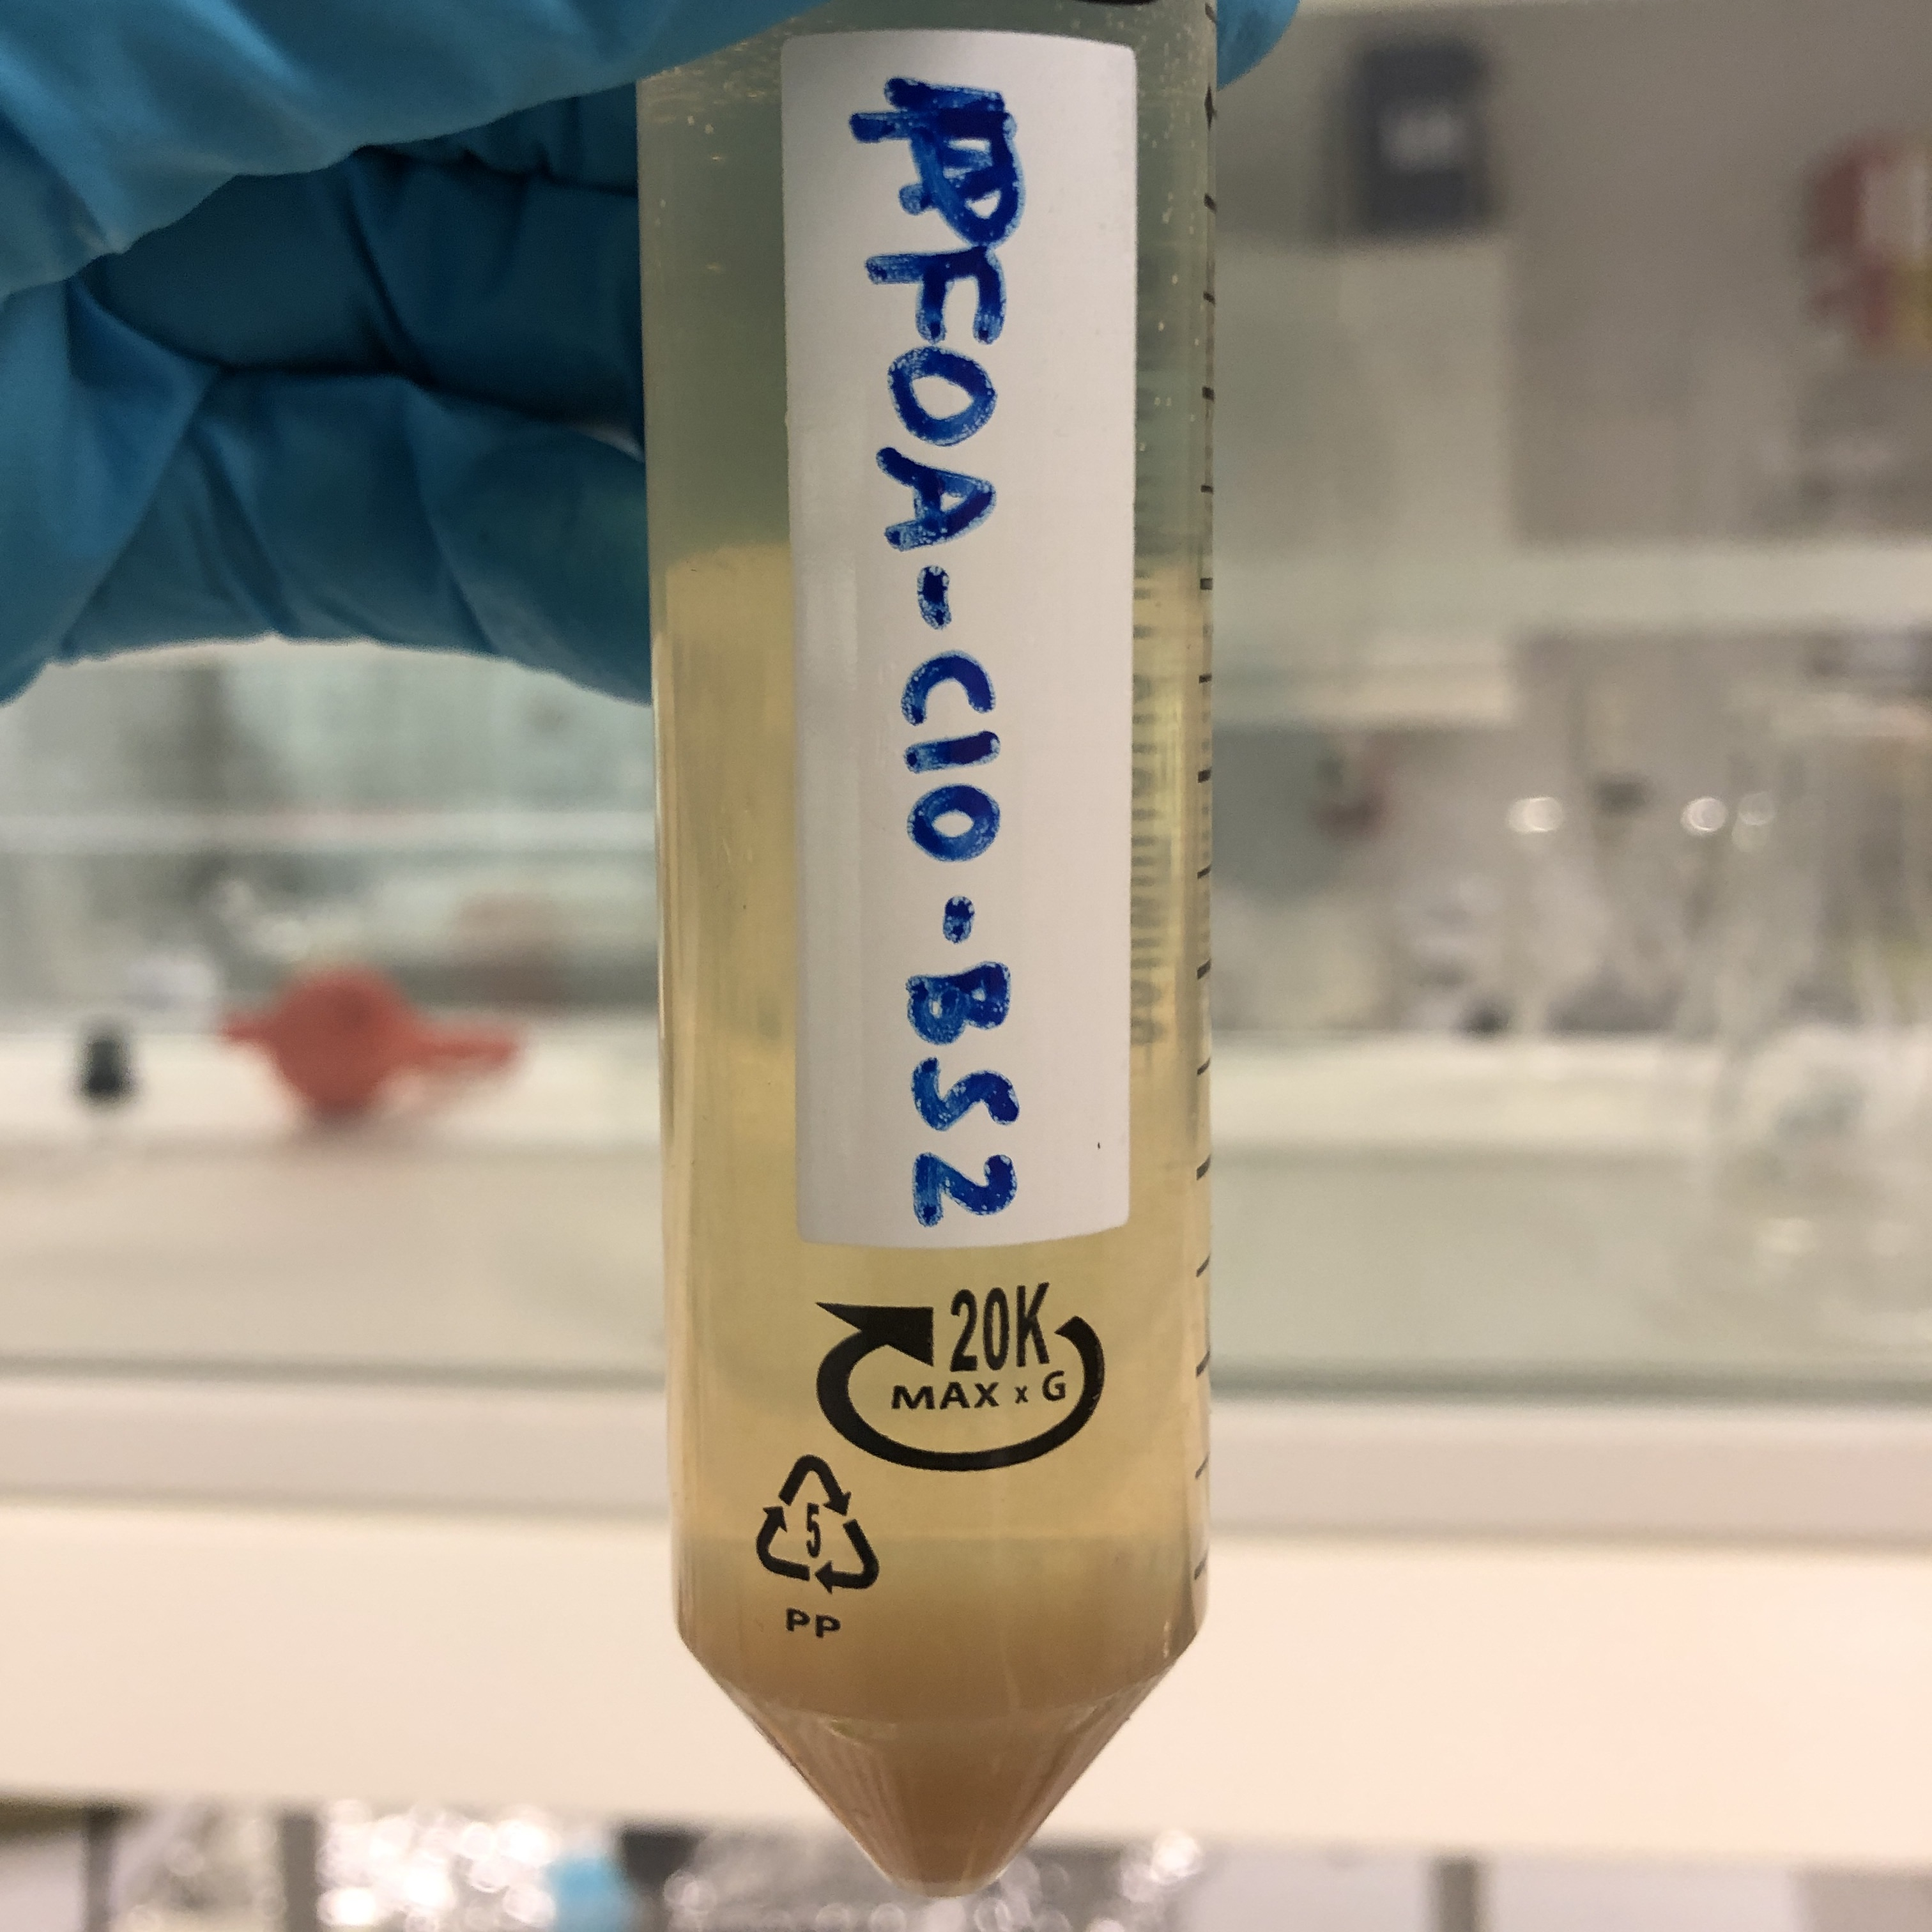
\includegraphics[width=0.6\linewidth,scale=0.6]{Bilder/Samples/Precipitation.jpg}
    \caption{Precipitation observed when filtered soil samples were adjusted to pH 3 with 1 M acetic acid.}
    \label{fig:precip}
\end{figure}

\section{Biochar properties}



\section{Sorption}





\section{Sustainability}
LCA (life cycle assessment), sustainability aspects of production of biochar
High operating energy and cost different technologies \citep{Alhashimi2017}


\section{Uncertainty}
\section{Uncertainty}
\subsubsection{Losses of PFAS to laboratory ware}
\citep{Lath2019labsorb}: 
Syringe filters: sorption of PFOA to centrifuge tubes and filter membranes. Sorption onto syringe surface: negligible due to short residence time (\textless 10 s). 74\% recovery from regenerated cellulose syringe filter. No improvement in recovery was seen when conditioning the syringe filters with phosphate solution or methanol. No trend between losses of PFOA on syringe filter and increasing spike concentrations. Centrifugation only is therefore advised if possible to avoid filtration losses. 

Test tubes: Greater recoveries from glass tubes than plastic, PP poorest recovery (55-68 \% recovery)... Contact time of PFAS residing in tubes for longer than 7 days should not be of significance, as \citep{Lath2019labsorb} propose that sorption and saturation of tube walls occur within hours. 74-81 \% recovery for PP when testing dependence on pH and ionic strength. Slight pH dependence, higher recovery at higher pH due to repulsion of negatively charged functional groups (PP has negative surface charge above pH 3.5-4. Bridging effect will be observed at higher pH's between cations like Ca2+, but is still considered negligible compared to the losses due to the physicochemical properties of the materials themselves. In general PP and plastics consists of mainly carbon hydrogen chains and are more hydrophobic than glassware. Sorption to tube walls saturate, so recoveries increase significantly with higher spike concentrations (e.g. for PP, 12-415 ug/L spiked PFOA increased recovery from 53.7-85.5 \%). Therefore, quantification of low concentrations may be subject to highest error, and in most cases will be an underestimation of dissolved concentrations. 

\subsection{Analytical uncertainty}

\subsubsection{Pipettes} 
The pipettes used for making the PFCA dilutions were calibrated. The three pipettes were: 1) 2-10 mL, 2) 200-1000 \textmu L, and 3) 5-50 \textmu L. All pipettes were below the permitted coefficient of variation (CV = 0.3, 0.5, and 2 $\%$ respectively (\cref{appSec:misclab}, \crefrange{appTab:pip2-10}{appTab:pip5-50}).

Since the diameter of the centrifuge tube (30 mm) was larger than that of a volumetric flask and biochar was added prior to the dilution process, the final concentration of the sorbent-sorbate mixture may have a heightened inaccuracy. However, the volume of which 0.1 g biochar occupies can be considered insignificant due to the high absorptive capacity of biochar and small mass used. Therefore a set of 10 centrifuge tubes filled to 50 mL containing 0.1 g CWC were weighed to control the uncertainty of the final dilutions. The results from weighing show that the weight of 10 trials were not accurate but precise, which means that all samples were prepared with the same final volume even though this volume deviates from 50 mL (\cref{appTab:PPcentrifuge}). 

\subsection{Representativeness}
Are the results representative of what goes on in real life? Sorption by shaking for 14 days represent an assumed equilibrium between PFCAs in the water and soil phase. A comparable situation in the field would be washing of the soil with large amounts of water such as during heavy rainfall. This will only be the case during occasional stormwater events and thus the results from this research could benefit from being supplemented with results from leaching tests using biochar mixed with soil. However, the relationship:

\begin{align}
    \frac{k_1}{k_2}
\end{align}

where \(k_1\) is the PFCA sorption (adsorption and absorption) rate and \(k_2\) is the PFCA desorption rate, where \(k_1>>k_2\), which indicates that sorption is many times higher, and in an equilibrium situation, sorption and desorption will be at steady state \citep{Cornelissen2005}. 

Uncertainty
Vel, du kan jo prøve å legge sammen alle de feilene. Det finnes jo forskjellige typer feilkilder i et stort forsøksoppsett. Det man ofte ser er at det er en eller to feil som er så store at de overskygger de andre. Da er det ikke noen vits å ta med alle de små. Feilen som ofte er størst er reproduserbarhet av metoden. Altså forskjellen mellom for eksempel prøver laget i triplikater. Det du kan gjøre i oppgaven din er jo å kort diskutere feilkildene du har og identifisere de største og viktigste.

Can make a table with key properties of feedstock, and pyrolysis parameters:
\begin{itemize}
\item moisture content
\item volatile matter
\item ash content
\item element composition (C, H, O)
\end{itemize}

\section{Feedstock and biochar}
\textit{CWC}\\
The yield was 38.7\%. 

\textit{ULS}\\
The yield was...\%.

\textit{BRL}\\
The yield was...\%.

\section{Biochar properties}
Biochar. 

\section{PFAS sorption to biochar}
Sorption. removal capacity of biochar (100-200 mg/g) \citep{Luo2021}

\subsection{Effect of sorbent type}
Sludge char.

\subsection{Effect of PFAS chain length and functional group}
Chain length matters. 

